\documentclass[output=paper, colorlinks, citecolor=brown, newtxmath]{langsci/langscibook}
\ChapterDOI{10.5281/zenodo.3764863}
%\bibliography{localbibliography}
%% add all extra packages you need to load to this file  
\usepackage{tabularx} 
\definecolor{lsDOIGray}{cmyk}{0,0,0,0.45}

\usepackage{xassoccnt}
\newcounter{realpage}
\DeclareAssociatedCounters{page}{realpage}
\AtBeginDocument{%
  \stepcounter{realpage}
}

%%%%%%%%%%%%%%%%%%%%%%%%%%%%%%%%%%%%%%%%%%%%%%%%%%%%
%%%           Examples                           %%%
%%%%%%%%%%%%%%%%%%%%%%%%%%%%%%%%%%%%%%%%%%%%%%%%%%%%  
%% if you want the source line of examples to be in italics, uncomment the following line
% \renewcommand{\exfont}{\itshape}
\usepackage{lipsum}
\usepackage{langsci-optional}
\usepackage{./langsci-osl}
\usepackage{langsci-lgr}
\usepackage{langsci-gb4e}
\usepackage{stmaryrd}
\usepackage{pifont} % needed for checkmark \ding{51} and cross \ding{55}
\usepackage[linguistics]{forest}

% ch06
\usepackage[euler]{textgreek}
% ch07
\usepackage{soul}
\usepackage{graphicx}
% ch08, ch14
\usepackage{multicol}
% ch11
\usepackage{fnpct}
% ch13
\usepackage{scrextend}
\usepackage{enumitem}
% ch14
\usepackage{tabto}
\usepackage{multirow}

\usepackage{langsci-cgloss}

%\newcommand{\smiley}{ :) }

% non-italics in examples

\renewcommand{\eachwordone}{\upshape}

% non-italics in examples in footnotes

\renewcommand{\fnexfont}{\footnotesize\upshape}
\renewcommand{\fnglossfont}{\footnotesize\upshape}
\renewcommand{\fntransfont}{\footnotesize\upshape}
\renewcommand{\fnexnrfont}{\fnexfont\upshape}

% chapter03 goncharov

\newcommand{\p}{\textsc{pfv\ }}
\newcommand{\im}{\textsc{ipfv\ }}

\makeatletter
\let\thetitle\@title
\let\theauthor\@author 
\makeatother

\newcommand{\togglepaper}[1][0]{  
  \addbibresource{../localbibliography.bib}  
  \papernote{\scriptsize\normalfont
    \theauthor.
    \thetitle. 
    To appear in: 
    Change Volume Editor \& in localcommands.tex 
    Change volume title in localcommands.tex
    Berlin: Language Science Press. [preliminary page numbering]
  }
  \pagenumbering{roman}
  \setcounter{chapter}{#1}
  \addtocounter{chapter}{-1}
}

\providecommand{\orcid}[1]{}
\IfFileExists{../localcommands.tex}{
  % add all extra packages you need to load to this file  
\usepackage{tabularx} 
\definecolor{lsDOIGray}{cmyk}{0,0,0,0.45}

\usepackage{xassoccnt}
\newcounter{realpage}
\DeclareAssociatedCounters{page}{realpage}
\AtBeginDocument{%
  \stepcounter{realpage}
}

%%%%%%%%%%%%%%%%%%%%%%%%%%%%%%%%%%%%%%%%%%%%%%%%%%%%
%%%           Examples                           %%%
%%%%%%%%%%%%%%%%%%%%%%%%%%%%%%%%%%%%%%%%%%%%%%%%%%%%  
%% if you want the source line of examples to be in italics, uncomment the following line
% \renewcommand{\exfont}{\itshape}
\usepackage{lipsum}
\usepackage{langsci-optional}
\usepackage{./langsci-osl}
\usepackage{langsci-lgr}
\usepackage{langsci-gb4e}
\usepackage{stmaryrd}
\usepackage{pifont} % needed for checkmark \ding{51} and cross \ding{55}
\usepackage[linguistics]{forest}

% ch06
\usepackage[euler]{textgreek}
% ch07
\usepackage{soul}
\usepackage{graphicx}
% ch08, ch14
\usepackage{multicol}
% ch11
\usepackage{fnpct}
% ch13
\usepackage{scrextend}
\usepackage{enumitem}
% ch14
\usepackage{tabto}
\usepackage{multirow}

\usepackage{langsci-cgloss}

  \newcommand{\smiley}{ :) }

% non-italics in examples

\renewcommand{\eachwordone}{\upshape}

% non-italics in examples in footnotes

\renewcommand{\fnexfont}{\footnotesize\upshape}
\renewcommand{\fnglossfont}{\footnotesize\upshape}
\renewcommand{\fntransfont}{\footnotesize\upshape}
\renewcommand{\fnexnrfont}{\fnexfont\upshape}

% chapter03 goncharov

\newcommand{\p}{\textsc{pfv\ }}
\newcommand{\im}{\textsc{ipfv\ }}

\makeatletter
\let\thetitle\@title
\let\theauthor\@author 
\makeatother

\newcommand{\togglepaper}[1][0]{  
  \addbibresource{../localbibliography.bib}  
  \papernote{\scriptsize\normalfont
    \theauthor.
    \thetitle. 
    To appear in: 
    Change Volume Editor \& in localcommands.tex 
    Change volume title in localcommands.tex
    Berlin: Language Science Press. [preliminary page numbering]
  }
  \pagenumbering{roman}
  \setcounter{chapter}{#1}
  \addtocounter{chapter}{-1}
}

\providecommand{\orcid}[1]{}
  %% hyphenation points for line breaks
%% Normally, automatic hyphenation in LaTeX is very good
%% If a word is mis-hyphenated, add it to this file
%%
%% add information to TeX file before \begin{document} with:
%% %% hyphenation points for line breaks
%% Normally, automatic hyphenation in LaTeX is very good
%% If a word is mis-hyphenated, add it to this file
%%
%% add information to TeX file before \begin{document} with:
%% %% hyphenation points for line breaks
%% Normally, automatic hyphenation in LaTeX is very good
%% If a word is mis-hyphenated, add it to this file
%%
%% add information to TeX file before \begin{document} with:
%% \include{localhyphenation}
\hyphenation{
Ro-ma-no-va
Isa-čen-ko
}

\hyphenation{
Ro-ma-no-va
Isa-čen-ko
}

\hyphenation{
Ro-ma-no-va
Isa-čen-ko
}

  \togglepaper[11]%%chapternumber
}{}
%\togglepaper[11]

\title{Negation, comparative and alternatives: Experimental evidence from Czech}

\author{Iveta Šafratová\affiliation{Masaryk University in Brno}}

\abstract{The semantic interplay of negation with focus and scalar implicatures influences acceptability judgments. This paper describes two readings of sentences with comparatives and negation, namely the equality reading and the interval reading. The experiment provides evidence that sentences with negated comparatives prefer the equality reading in Czech. I argue that Czech negated comparatives result in the preferential equality reading as do English negated comparatives; but I challenge the claim that Czech negation  \textit{ne} `no' activates focus alternatives, unlike in English negated comparatives with \textit{no} where scalar alternatives cause the equality reading. I argue that focus alternatives and scalar alternatives are the same. Both Czech  \textit{ne-} `not' and English  \textit{not} in verbal negation comparatives lead to the preferential equality reading if negation has narrow scope over the maximality operator.

\keywords{constituent negation; verbal negation; scalar implicatures; focus alternatives; comparative; Czech; experimental semantics}
}


\begin{document}
\maketitle

%(like \textit{no more than/not more than})
\il{Czech|(}
\section{Introduction}

In recent years, the topic of scalar implicatures and numerals has attracted considerable attention, and the research gave rise to several influential theories (\citealt{larson1988scope,krifka1999least,sauerland2004scalar,fox2006universal}, among others). This article investigates how \isi{negation} interacts with comparatives involving numerals. I will \isi{focus} on the comparison of \ili{English} data with \ili{Czech}. Though the semantics of many different types of \ili{Slavic} numerals have recently been explored with considerable success  \citep[e.g.][]{docekal2013numerals,wagiel2014boys,wagiel2015sums}, so far little attention has been dedicated to their behavior in the interaction with \isi{negation} and comparatives (with the notable exceptions of \citealt{dovcekal2017upper} and \citealt{docekal_wagiel2018event} respectively). In this paper, I intend to shed new light on this topic by means of experimental investigation.

The article investigates how \isi{negation} interacts with comparatives. We start with Rick Nouwen's observation about \ili{English} negated comparatives \citep{nouwen2008upper}. He distinguishes two sub-types of comparatives, i.e., strict comparatives (\textit{-er}) in \REF{ex:mush} and non-strict comparatives (\textit{no(t) -er}) in \REF{ex:no_mush}.

\ea \ea John found more than 20 mushrooms.\label{ex:mush}
\ex John found no more than 20 mushrooms.\label{ex:no_mush}
\z
\z

\noindent Strict comparatives express either the relation \textit{less} or \textit{more}. We would expect that the only thing non-strict comparatives do is that they simply reverse the relation.
But, according to \cite{nouwen2008upper}, \isi{negation}
changes the relation from $>$ to $\leq$ and from $<$ to $\geq$. Non-strict comparatives are ambiguous due to
their ability to express either \textit{less/more} or \textit{equality}.

Non-strict comparatives can be negated either by constituent \isi{negation} (\textsc{cn}), as in \REF{ex:mush_cn}, or by \isi{verbal negation} (\textsc{vn}), as in \REF{ex:mush_vn}.

\ea \ea John found no more than 20 mushrooms.\label{ex:mush_cn}
\ex John did not find more than 20 mushrooms.\label{ex:mush_vn}
\z
\z


\noindent We \isi{focus} on whether these two types of \isi{negation} (\textsc{vn/cn}) influence the ambiguity of non-strict comparatives and whether the composition of the meaning of non-strict comparatives happens in the same way in \ili{English} and \ili{Czech}.



\subsection{English non-strict comparatives}

A sentence with a \isi{comparative} activates scalar alternatives. Scalar alternatives are present in scalar implications developed by \cite{horn1989natural,horn1996presupposition}, they are a subtype of generalized conversational \isi{implicature} associated with scalar values ordered from the weakest value to the strongest value \citep{horn20135}. Consider the following sample sentences with their \isi{scalar implicature} (\isi{SI}).

\ea Some people left.\\
\isi{SI}: $\neg\,$all people left
\z

\ea John has two children.\\
\isi{SI}: $\neg\,$John has three children
\z

\ea John bought a book or a pen.\\
\isi{SI}: $\neg\,$John bought a book and a pen
\z


\noindent The strict \isi{comparative} \REF{ex:str} and the non-strict \isi{comparative} \REF{ex:non_str} both lead to scalar implications, but with a different result.

\ea \ea John found more than 20 mushrooms.\label{ex:str}
\ex John found no more than 20 mushrooms.\label{ex:non_str}
\z
\z

\noindent The strict \isi{comparative} in \REF{ex:str} means that the  minimum number of mushrooms is more than 20. The limit lies in the lower bound, but the upper bound is unbounded, i.e. (20,$\infty$).

\ea John found more than 20 mushrooms.
\ea truth conditions: $\cnst{max}_{\cnst{d}}\big(\lambda y\exists x[\#x=y \wedge \textsc{mushroom}(x) \wedge \textsc{find}(\textsc{John},x)]\big) > 20$
\z
\z


\noindent The \isi{negation} reverses the relation from $>$ to $\leq$; therefore the non-strict \isi{comparative} in \REF{ex:non_str} means that the maximum number of mushrooms is 20. The limit lies in the upper bound, whereas the lower bound is not specified, but the natural perception of the world limits the minimal number, i.e., (0,20).

\cite{nouwen2008upper} explains the composition of non-strict comparatives. According to him, the non-strict \isi{comparative} in \REF{ex:non_str} has two readings: the \isi{interval reading} corresponds to the relation \textit{less} -- (0,20) and the \isi{equality reading} corresponds to the \textit{equality} relation -- (0,20).

If constituent \isi{negation} negates a \isi{comparative} (\textsc{cn-}\isi{comparative}), as in \REF{ex:sen}, the \isi{equality reading} results from the strengthening of the truth condition interpretation via \isi{scalar implicature}. The sentence has standard truth conditions \REF{ex:tc_1} and also scalar implicatures \REF{ex:si_1}, \REF{ex:si_1_2}, etc., but scalar implicatures are negated because the proposition stating the number of mushrooms is $\leq$ 19 is logically stronger than the proposition stating the same number is $\leq$ 20.\footnote{Logical strength relates to the \isi{entailment}. The proposition \textit{John didn't find 19 mushrooms} entails the proposition \textit{John didn't find 20 mushrooms}; therefore the first proposition is stronger than the second proposition.

\ea John didn't find 19 mushrooms $\rightarrow$ John didn't find 20 mushrooms $\rightarrow$ \dots
\zlast} The \isi{equality reading} then arises from the denial of scalar implicatures and strengthening of truth conditions.

\ea \label{ex:sen} John found no more than 20 mushrooms.
        \ea truth conditions: $\cnst{max}_{\cnst{d}}(\lambda d\,.\,$the number of mushrooms was $d\leq 20)$ \label{ex:tc_1}
		\ex \isi{SI}: $\neg\cnst{max}_{\cnst{d}}(\lambda d\,.\,$the number of mushrooms was $d\leq 19)$ \label{ex:si_1}
		\ex \isi{SI}: $\neg\cnst{max}_{\cnst{d}}(\lambda d\,.\,$the number of mushrooms was $d\leq 18)$ \label{ex:si_1_2}
\ex $\cnst{max}_{\cnst{d}}(\lambda d\,.\,$the number of mushrooms was $d=20)$
\z
\z


\noindent \cite{nouwen2008upper} claims that the most salient interpretation of \ili{English} \textsc{cn-}com\-par\-a\-tives is the \isi{equality reading}, but he doesn't exclude the \isi{interval reading}.\footnote{The \isi{interval reading} arises because scalar implicatures need not be drawn, and the strengthening of truth conditions doesn't occur.}

If \isi{verbal negation} negates a \isi{comparative} (\textsc{vn-}\isi{comparative}), as in \REF{ex:ver}, both readings are also possible but due to different reasons than in \textsc{cn-}comparatives. \cite{nouwen2008upper} claims that interval and equality readings arise because \isi{verbal negation} can take two scopes within the proposition: narrow scope, as in \REF{ex:eng_exh}, which corresponds to \REF{ex:tc_1}, and wide scope, as in \REF{ex:eng_int}.

\ea  \label{ex:ver} John did not find more than 20 mushrooms.
	\ea $\cnst{max}_{\cnst{d}}\big(\lambda y\exists x[\#x=y \wedge \textsc{mushroom}(x) \wedge \textsc{find}(\textsc{John},x)]\big) \leq 20$ \label{ex:eng_exh}
	\ex $\neg\cnst{max}_{\cnst{d}}\big(\lambda y\exists x[\#x=y \wedge \textsc{mushroom}(x) \wedge \textsc{find}(\textsc{John},x)]\big) > 20$ \label{ex:eng_int}
\z
\z

\noindent The narrow scope leads to scalar alternatives. As in the \textsc{cn-}comparatives, the scalar alternatives are negated, and the strengthening of truth conditions causes the \isi{equality reading}. The wide scope is interpreted as a denial and truth conditions of the proposition are weaker: `it is not true that John found more than 20 mushrooms'. Strengthening does not occur in the construction because no scalar alternatives are present; therefore only the \isi{interval reading} is possible. Nouwen argues that sentences with \textsc{vn-}comparatives show a preference for the \isi{interval reading}.

\tabref{tab:1:eng_comp} summarizes Nouwen's observations of \ili{English} negated comparatives.

\begin{table}
\caption{English negated comparatives}
\label{tab:1:eng_comp}
 \begin{tabular}{lll}
  \lsptoprule
  \textsc{cn-}comparatives & \isi{equality reading} & preferred\\
  \textsc{cn-}comparatives & \isi{interval reading} & non-preferred\\
   \textsc{vn-}comparatives (wide scope) & \isi{interval reading} & preferred\\
    \textsc{vn-}comparatives (wide scope) & \isi{equality reading} & non-preferred\\
  \textsc{vn-}comparatives (narrow scope) & \isi{equality reading} & preferred\\
  \textsc{vn-}comparatives (narrow scope) & \isi{interval reading} & non-preferred\\
\lspbottomrule

  \end{tabular}
  \end{table}


\tabref{tab:1:eng_comp} shows a nice pattern of \ili{English} negated comparatives, i.e., \textsc{cn-}com\-par\-a\-tives prefer the \isi{equality reading}, whereas \textsc{vn-}comparatives prefer the \isi{interval reading} if \isi{verbal negation} takes wide scope over the maximality operator. The \isi{equality reading} is preferred in the case of narrow scope of \isi{verbal negation}. I now contrast this observation with \ili{Czech} negated comparatives.


\subsection{Czech non-strict comparatives}

While \ili{English} \textsc{cn} \textit{no} and \textsc{vn} \textit{not} differ morphologically,  \ili{Czech} \textsc{cn} and \textsc{vn} share the same morphological form \textit{ne}, but its semantic and syntactic properties vary. The marker of \textsc{cn} is a free morpheme; it stands independently in a sentence, as in \REF{ex:cz_cn}. The marker of \textsc{vn} is an ordinary prefixal \isi{verbal negation}; it firmly connects to a lexical \isi{verb} or an auxiliary, as in \REF{ex:cz_vn}.

\ea
\gll Chci být doktorem, ne učitelem.\\
want.\textsc{prs.1sg} be.\textsc{inf} doctor.\textsc{ins.sg} not teacher.\textsc{ins.sg}\\
\glt `I want to be a doctor, not a teacher.' \label{ex:cz_cn}
\z

\ea
\gll Nechci být učitelem.\\
\textsc{neg}.want.\textsc{prs.1sg} be.\textsc{inf} teacher.\textsc{ins.sg}\\
\glt `I don't want to be a teacher.' \label{ex:cz_vn}
\z


\noindent \cite{dovcekal2017upper} investigates non-strict comparatives in \ili{Slavic} languages, especially in \ili{Czech}. Following the previous investigation (\citealt{jasinskaja2016information}, among others), Dočekal starts with an observation that \ili{Slavic} \isi{focus} particles have to c-command their \isi{focus} marked constituents \REF{ex:only_c}, and they have to be adjacent to the \isi{focus} marked constituent, unlike \ili{English} \isi{focus} particles \REF{ex:only_e}.\footnote{\cite{dovcekal2017upper} gives examples with the \ili{Czech} prototypical \isi{focus} particle \textit{pouze} `only' and he claims that \ili{Czech} \textsc{cn} behaves the same way.} In this respect, \ili{Slavic} \isi{focus} particles resemble \ili{German} \isi{focus} particles (see \citealt{buring2001v3}).

\ea \label{ex:only_c}
 \ea \gll Tento slovník překládá \minsp{\{} pouze / ne\} \minsp{[} z angličtiny]$_{\textsc{foc}}$ do svahilštiny.\\
    this.\textsc{nom.sg} dictionary.\textsc{nom.sg} translate.\textsc{prs.1sg} {} only {} not {} from \ili{English}.\textsc{gen.sg} to \ili{Swahili}.\textsc{gen.sg}\\
    \glt `This dictionary translates only/not from \ili{English} to \ili{Swahili}.'
\ex
    \gll Tento slovník překládá z angličtiny pouze \minsp{[} do svahilštiny]$_{\textsc{foc}}$.\\
    this.\textsc{nom.sg} dictionary.\textsc{nom.sg} translate.\textsc{prs.1sg} from \ili{English}.\textsc{gen.sg} only {} to \ili{Swahili}.\textsc{gen.sg}\\
    \glt `This dictionary translates from \ili{English} to \ili{Swahili} only.' \label{ex:only_c_2}
\ex
    \gll Tento slovník překládá z angličtiny ne \minsp{[} do svahilštiny]$_{\textsc{foc}}$.\\
    this.\textsc{nom.sg} dictionary.\textsc{nom.sg} translate.\textsc{prs.1sg} from \ili{English}.\textsc{gen.sg} not {} to \ili{Swahili}.\textsc{gen.sg}\\
    \glt `This dictionary translates from \ili{English} not to \ili{Swahili}.' \label{ex:only_c_3}
\z
\z


\ea \label{ex:only_e}
	\ea I behave only [seriously]$_{\textsc{foc}}$.
    \ex I only behave [seriously]$_{\textsc{foc}}$.\hfill\citep{dovcekal2017upper}
\z
\z


\noindent Based on the pattern demonstrated above, \cite{dovcekal2017upper} concludes that \ili{Czech} \textsc{cn} is a \isi{focus} particle, unlike \ili{English} \textsc{cn}. Negated comparatives activate alternatives in both languages, but the type of alternatives differs: scalar alternatives in \ili{English} \citep{nouwen2008upper} and \isi{focus} alternatives in \ili{Czech} \citep{dovcekal2017upper}.

We interpret the semantics of \isi{focus} by the proposal of \cite{rooth1985association,rooth1992theory}: each sentence with \isi{focus} has two semantic values: ordinary value $\llbracket \alpha
 \rrbracket^{o}$ and \isi{focus} value $\llbracket \alpha \rrbracket^{f}$. Ordinary value is the truth-conditional value of $\alpha$; \isi{focus} value is the set of alternatives of $\alpha$, as in \REF{ex:set}. Focus sensitive operators bear existential presuppositions of \isi{focus} alternatives. The existential \isi{presupposition} means that at least one alternative from the set of alternatives is true (see \citealt{rooth1985association,rooth1992theory}).

\ea \ea Charles gave a rose to [Mary]$_{\textsc{foc}}$.
	\ex \{Charles gave a rose to $x$ | $x$ is a person\}
    \label{ex:set}
\z
\z


\noindent \textsc{cn} adds the $\neg$ operator to a sentence; it negates the assertion and presupposes that at least one alternative is true, as in \REF{ex:hammer}. The assertion is negated \REF{ex:negham}, but the constituent \isi{negation} -- being a \isi{focus} particle -- introduces the \isi{presupposition} in \REF{ex:presham} (which is satisfied by \textit{a hoe}).

\ea  Maxwell killed the judge not with [a hammer]$_{\textsc{foc}}$, but with [a hoe]$_{\textsc{foc}}$. \label{ex:hammer} \ea $\neg\,$Maxwell killed the judge with a hammer \label{ex:negham}
\ex Presupposition: $\exists x[$Maxwell killed the judge with $x]$ \label{ex:presham}
\z
\z

\noindent \cite{dovcekal2017upper} selected and classified sentences with \textsc{cn} from the largest corpus of contemporary \ili{Czech}, SYN2010. He formalizes the negated \isi{focus} marked constituent cross-categorically because \ili{Czech} \textsc{cn} may modify various types of constituents, e.g., PP, AP, NumP, AdvP.\footnote{\label{footn:expl}According to \cite{dovcekal2017upper}, Nouwen's explanation via negated scalar implicatures would not work for \ili{Czech} because \ili{Czech} \textsc{cn} modifies various types of constituents, not only numerical phrases. A compromise would be to say that in \ili{Czech} \textsc{cn-}comparatives activate both scalar alternatives and \isi{focus} alternatives.}

The standard consideration about \isi{focus} is that both the ordinary value and the \isi{focus} value have to be of the same semantic type. We illustrate this in example \REF{ex:doktor}: both constituents \textit{a doctor} and \textit{a teacher} are of type $\stb{e,t}$ and in this case are predicates. They have to share the same property because they belong to the set of alternatives (in this case professions). The ordinary value \textit{a teacher} is negated by \textsc{cn}, and the \isi{focus} value \textit{a doctor} satisfies the need for at least one alternative to be true.

\ea \label{ex:doktor} \gll Chci být doktorem, ne učitelem.\\
want.\textsc{prs.1sg} be.\textsc{inf} doctor.\textsc{ins.sg} not teacher.\textsc{ins.sg}\\
	\glt `I want to be a doctor, not a teacher.'
    \ea ordinary value: a teacher
    \ex \isi{focus} value: a doctor
\z
\z

\noindent Dočekal proposes that the \ili{Czech} \isi{focus} operator \textsc{cn} targets the \isi{comparative} morpheme \textit{více než} `no more' that has the following possible alternatives: $\leq, =, >$. At least one alternative must be valid. The alternative $>$ is negated; therefore two alternatives remain: the alternative = leads to the \isi{equality reading}, as in \REF{ex:exh_beer}, the alternative $\leq$ leads to the \isi{interval reading}, as in \REF{ex:int_beer}.

\ea Peter drank no [more than] 5$_{\textsc{foc}}$ beers yesterday.
	\ea the \isi{equality reading}: Peter drank no more, but exactly 5 beers. \label{ex:exh_beer}
	\ex the \isi{interval reading}: Peter drank not more, but less than 5 beers or equal. \label{ex:int_beer}
\z
\z

\noindent Both \ili{Czech} \textsc{cn-} and \textsc{vn-}comparatives are ambiguous between interval and \isi{equality reading}, but \cite{dovcekal2017upper} expresses the intuition that \ili{Czech} \textsc{cn-}com\-par\-a\-tives prefer the \isi{interval reading}, whereas \textsc{vn-}comparatives prefer the \isi{equality reading}.\footnote{\cite{dovcekal2017upper} has verified his intuition with a small corpus study; he has checked whether a context of the sentences approves the \isi{interval reading} or the \isi{equality reading}. Also, he has consulted the translation of a sample sentence with native speakers of \ili{Polish}, \ili{Bulgarian} and \ili{Russian}. Based on the corpus study and the consultations with several native speakers of \ili{Slavic} languages, Dočekal argues that \textsc{cn-}comparatives prefer the \isi{interval reading} in \ili{Czech}. He describes \textsc{vn-}comparatives only minimally, he mainly investigates \textsc{cn-}comparatives.
} \tabref{tab:2:cz_comp} summarizes Dočekal's observations of \ili{Czech} \textsc{cn-} comparatives.

\begin{table}
\caption{Czech negated comparatives}
\label{tab:2:cz_comp}
 \begin{tabular}{lll}
  \lsptoprule
    \textsc{cn-}comparatives & \isi{interval reading} & preferred\\
  \textsc{cn-}comparatives & \isi{equality reading} & non-preferred\\
   \textsc{vn-}comparatives & \isi{equality reading} & preferred\\
  \textsc{vn-}comparatives & \isi{interval reading} & non-preferred\\  \lspbottomrule
  \end{tabular}
  \end{table}


Following Dočekal, I hypothesize that \ili{Czech} \textsc{cn-}comparatives show a preference for the \isi{interval reading} and \textsc{vn-}comparatives show a preference for the \isi{equality reading}, although \ili{Czech} \textsc{vn-}comparatives have been less explored concerning ambiguity than \textsc{cn-}comparatives.

A comparison of \tabref{tab:1:eng_comp} and \tabref{tab:2:cz_comp} shows that \ili{English} \textsc{cn-}com\-par\-a\-tives prefer the \isi{equality reading}, whereas \ili{Czech} \textsc{cn-}comparatives prefer the \isi{interval reading}. The \isi{verbal negation} can take two possible scopes. When \ili{English} \isi{verbal negation} is construed with wide scope, there is a preference for the \isi{interval reading}, but the \isi{equality reading} is preferred when \isi{verbal negation} takes narrow scope. An observation of \ili{Czech} \isi{verbal negation} is not divided into two possible scopes, the summary is only such that \ili{Czech} \textsc{vn-}comparatives prefer the \isi{equality reading}.

The preference for the \isi{interval reading} or the \isi{equality reading} of \ili{Czech} negated comparatives is just Dočekal's hypothesis; therefore it would be appropriate to verify it experimentally. Before introducing an experiment, we will use the remainder of this section to present another approach to alternatives.\footnote{Thanks to an anonymous reviewer for raising this point.}

We argue so far that the difference between \ili{English} negated comparatives and \ili{Czech} negated comparatives comes from different alternatives. According to \cite{nouwen2008upper}, \ili{English} constituent \isi{negation} involves scalar alternatives, but for \cite{dovcekal2017upper}, \ili{Czech} constituent \isi{negation} \textit{ne} is a \isi{focus} particle; therefore \ili{Czech} constituent \isi{negation} works with \isi{focus} alternatives. Focus alternatives differ from scalar alternatives in the fact that scalar alternatives are ordered on a scale from the weakest alternative to the strongest one, whereas \isi{focus} alternatives are not hierarchically ranked because they are on the same level.

In recent years, the distinction between scalar alternatives and \isi{focus} alternatives faces doubts (see \citealt{katzir2007structurally,fox2011characterization,fox2018economy}). Both scalar alternatives and \isi{focus} alternatives are considered to be determined in the same way, namely as a contextual restriction of the \isi{focus} value of the sentence. Based on that, alternatives are in a particular logical relationship with the assertion or the prejacent. A unified nature of scalar and \isi{focus} alternatives goes against standard type-theoretic definitions of \isi{focus} values \citep{fox2011characterization}. For \citet{krifka1995semantics}, scalar items are inherently focused and their alternatives are scales. The revised theory of scalar and \isi{focus} alternatives challenges Dočekal's assertion that Nouwen's explanation for \ili{English} \textsc{cn-}comparatives cannot work for \ili{Czech} \textsc{cn-}comparatives because, according to \citet{dovcekal2017upper}, negated comparatives in \ili{Czech} activate a different type of alternatives, unlike in \ili{English}.

As I indicated before (see footnote \ref{footn:expl}), if we keep the distinction between scalar and \isi{focus} alternatives, we have to say that \ili{Czech} \textsc{cn-}comparatives activate both types of alternatives. An approach unifying these two types of alternatives into one group provides a more comprehensive view of the topic of alternatives.


\section{Experiment}

I experimentally tested the availability of two readings of negated comparatives in \ili{Czech}. I \isi{focus} on (i) whether both \textsc{cn-} and \textsc{vn-}comparatives are ambiguous between the equality and interval readings, and (ii) whether as predicted by the initial hypothesis \textsc{cn-}comparatives show a preference for the \isi{interval reading}, whereas \textsc{vn-}comparatives show a preference for the \isi{equality reading}.

\subsection{Method}

\subsubsection{Materials}

The experiment consisted of a truth value judgment task that tested to what extent \ili{Czech} native speakers accept sentences with \textsc{cn-}comparatives \textit{ne víc} `no more' and \textsc{vn-}comparatives \textit{ne $+$ \textsc{verb} víc} `not \textsc{verb} more' with respect to two possible interpretations: the \isi{equality reading} and the \isi{interval reading}.\footnote{The constituent \isi{negation} \textit{ne} `no' stands alone in a sentence, whereas the pre-\isi{verbal negation} \textit{ne-} `not' must be connected to a \isi{verb}.}

The experiment tested whether a sentence fits a given context. The context preceded the target sentence. Participants were instructed to answer either ``yes'' (\textit{věta je v daném kontextu pravdivá a vhodná} `the sentence is true and appropriate in the given context') or ``no'' (\textit{věta není v daném kontextu pravdivá a vhodná} `the sentence is not true and appropriate in the given context').\footnote{I agree with an anonymous reviewer that a weaker (interval) reading is true in the \isi{equality context}, but presumably less natural (acceptable). If a participant prioritizes the truth over naturalness, \textsc{cn}-comparatives, which would be judged unnatural in the \isi{equality context} according to the initial hypothesis, receive an answer ``yes'' in the equality condition because  \textsc{cn-}comparatives are true in the \isi{equality context}. The weaker reading is also true in the \isi{interval context}, but more natural. Even if a participant prioritizes the truth or naturalness, the answer should be ``yes.'' But \figref{fig:graf} shows that participants answered ``no'' more often: the \isi{interval reading} is less acceptable in the \isi{interval context} than in the \isi{equality context}.}

The experiment focused on these main issues:

\begin{itemize}
\item the interaction between a \isi{comparative} and the constituent \isi{negation}: \textit{ne} $+$ more `no' (\textsc{cn})
\item the interaction between a \isi{comparative} and the \isi{verbal negation}: \textit{ne-} $+$ a \isi{verb} `not' (\textsc{vn})
\end{itemize}

\noindent I investigated whether the \isi{syntactic position} of comparatives could influence the acceptability of sentences; therefore \isi{comparative} constructions in tested sentences appeared in two types of syntactic environment: (\textsc{a}) in a \isi{predicate position} and (\textsc{b}) in an \isi{object position}. Sentences in the experiment did not include comparatives in a \isi{subject position}. The support for choosing the two positions (predicate and object) follows from Nirit Kadmon's theory \citep{kadmon2001formal} that claims that the readings can differ in these two positions. I omitted the interaction between topic and \textsc{cn-/vn-}comparatives.

I tested the acceptability of each sentence in two contextual environments:  equality (\textsc{e}) and interval (\textsc{n}).

Consequently, I tested the acceptability of negated comparatives in eight conditions:
\begin{enumerate}
\item \textsc{ocne} -- \textsc{cn-}\isi{comparative} in an \isi{object position} against the \isi{equality context} \label{ex:item1}
\item \textsc{ocnn} -- \textsc{cn-}\isi{comparative} in an \isi{object position} against the \isi{interval context}
\item \textsc{ovne} -- \textsc{vn-}\isi{comparative} in an \isi{object position} against the \isi{equality context}
\item \textsc{ovnn} -- \textsc{vn-}\isi{comparative} in an \isi{object position} against the \isi{interval context}
\item \textsc{pcne} -- \textsc{cn-}\isi{comparative} in a \isi{predicate position} against the \isi{equality context}
\item \textsc{pcnn} -- \textsc{cn-}\isi{comparative} in a \isi{predicate position} against the \isi{interval context}
\item \textsc{pvne} -- \textsc{vn-}\isi{comparative} in a \isi{predicate position} against the \isi{equality context}
\item \textsc{pvnn} -- \textsc{vn-}\isi{comparative} in a \isi{predicate position} against the \isi{interval context} \label{ex:item8}
\end{enumerate}

\noindent There were 16 items -- each item had 8 conditions (i.e., 128 sentences) -- and there were 16 fillers. Each participant judged 16 items and 16 fillers and the order of stimuli was randomized.\footnote{I used functions \textit{shuffle sequence} and \textit{rshuffle} in a statistical analysis. The functions are defined as randomizing and sequencing operations over an array of items in the Ibex manual.} The experiment was compiled from items and conditions in such a way that each item appeared only once in the experiment, whereas individual conditions cycled (repeated Latin-square design). All items were tested in all eight conditions \ref{ex:item1}--\ref{ex:item8} presented above.

Below, two sample items are shown: an item with \textsc{cn-}\isi{comparative} in a \isi{predicate position} in \REF{ex:pcn} and an item with \textsc{vn-}\isi{comparative} in a \isi{predicate position} in \REF{ex:pvn}. Items were tested against two contexts: either against the \isi{equality context} in \REF{ex:wine_e} or against the \isi{interval context} \REF{ex:wine_n} (not against both contexts simultaneously).


\ea
\gll Petr nalil víno do všech 6 sklenic.\\
Petr.\textsc{nom} pour.\textsc{pst.1sg} wine.\textsc{acc.sg} into all.\textsc{gen.pl} 6 glass.\textsc{gen.pl}\\\hfill\framebox{\textsc{e}}
\glt `Petr poured wine into all 6 glasses.' \label{ex:wine_e}
\z


\ea
\gll Petr nalil víno do všech 5 sklenic.\\
Petr.\textsc{nom} pour.\textsc{pst.1sg} wine.\textsc{acc.sg} into all.\textsc{gen.pl} 5 glass.\textsc{gen.pl}\\\hfill\framebox{\textsc{n}}
\glt `Petr poured wine into all 5 glasses.' \label{ex:wine_n}
\z

\ea
\gll Na stole je ne víc než 6 sklenic.\label{ex:pcn}\\
on table.\textsc{loc.sg} be.\textsc{prs.1sg} no more than 6 glass.\textsc{gen.pl}\\\hfill \framebox{\textsc{pcn}}
\glt `There are no more than 6 glasses on the table.'
\z

\ea
\gll Na stole není víc než 6 sklenic.\label{ex:pvn}\\
on table.\textsc{loc.sg} \textsc{neg}.be.\textsc{prs.1sg} more than 6 glass.\textsc{gen.pl}\\\hfill \framebox{\textsc{pvn}}
\glt `There are not more than 6 glasses on the table.'
\z


\noindent The other two sample items are following: an item with \textsc{cn-}\isi{comparative} in an \isi{object position} in \REF{ex:ocn} and an item with \textsc{vn-}\isi{comparative} in an \isi{object position} in \REF{ex:ovn}. Again, items were tested against two contexts: either against the \isi{equality context} in \REF{ex:rose_e} or the \isi{interval context} \REF{ex:rose_n}.

\ea
\gll Všech 6 růží bylo červených.\\
all.\textsc{gen.pl} 6 rose.\textsc{gen.pl} be.\textsc{pst.1sg} red.\textsc{gen.pl}\\\hfill\framebox{\textsc{e}}
\glt `All 6 roses were red.'  \label{ex:rose_e}
\z

\ea
\gll Všech 5 růží bylo červených.\\
all.\textsc{gen.pl} 5 rose.\textsc{gen.pl} be.\textsc{pst.1sg} red.\textsc{gen.pl}\\\hfill\framebox{\textsc{n}}
\glt `All 5 roses were red.'  \label{ex:rose_n}
\z

\ea
\gll Jan dal Marii k narozeninám ne víc než 6 růží.\label{ex:ocn}\\
John.\textsc{nom} give.\textsc{pst.1sg} Mary.\textsc{dat} to birthday.\textsc{dat.pl} no more than 6 rose.\textsc{gen.pl}\\\hfill \framebox{\textsc{ocn}}
\glt `John gave Mary no more than 6 roses for her birthday.'
\z

\ea
\gll Jan nedal Marii k narozeninám víc než 6 růží.\label{ex:ovn}\\
John.\textsc{nom} \textsc{neg}.give.\textsc{pst.1sg} Mary.\textsc{dat} to birthday.\textsc{dat.pl} more than 6 rose.\textsc{gen.pl}\\\hfill\framebox{\textsc{ovn}}
\glt`John didn't give Mary more than 6 roses for her birthday.'
\z


\noindent Each sentence is potentially ambiguous between the \isi{interval reading} and the \isi{equality reading}, but I assumed a preference for a particular reading. As predicted by the initial hypothesis, I expected that sentences with \textsc{cn-}comparatives like \REF{ex:pcn} and \REF{ex:ocn} will be more acceptable in the interval scenario, as in \REF{ex:wine_n} and \REF{ex:rose_n}, whereas sentences with \textsc{vn-}comparatives like \REF{ex:pvn} and \REF{ex:ovn} will be more acceptable in the equality scenario, as in \REF{ex:wine_e} and \REF{ex:rose_e}.

\subsubsection{Procedure and participants}
The experiment was run on Ibex and participants completed the experiment online. The experiment began with instructions and following that, the practice items and the truth value judgment and appropriateness task were presented.\footnote{The terms \textit{true} and \textit{false} are technical terms of logic and linguistics but the experiment targeted native speakers of \ili{Czech} irrespective of their academic background; therefore I used \textit{adequate} in the introduction.}\footnote{Follow the link below for the instructions and practice items, items and fillers used in the experiment: \href{https://github.com/ivetasafratova/Negation-comparative-and-alternatives-Experimental-evidence-from-Czech.git}{GitHub}}.
Participants were asked for the acceptability of a sentence against a context. 52 native speakers of \ili{Czech} participated in the experiment, mainly students from Masaryk University.


\subsection{Results}
The fillers in the acceptability task were either uncontroversially grammatical or ungrammatical, and I checked whether the average of each participant’s responses to ungrammatical fillers was lower than the average of his or her responses to grammatical fillers. Eight participants had to be excluded due to their unsuccessful scores in fillers; therefore I kept 44 subjects for subsequent analysis.

I designed the truth value judgment task using a mixed-effects linear model. To model the data I constructed 4 linear models (the standard lm command of R) of the acceptability of the 4 conditions as depending on their \textsc{e/n} sub-conditions. The equality condition was taken as the reference level for each condition (\textsc{pcn, pvn, ocn, ovn}).

For all four conditions the linear model summary resulted in a statistically significant difference between \textsc{e} and \textsc{n} sub-conditions: the mean acceptability was a response vector depending on the \textsc{e/n} as a predictor. The statistical outcome was the following:\footnote{The value \textit{t} states how big a difference there is between the \isi{equality reading} and the \isi{interval reading}, the value \textit{p} expresses how likely it is that the difference between the \isi{equality reading} and the \isi{interval reading} is random.}

\begin{enumerate}
\item \textsc{cn-}\isi{comparative} in a \isi{predicate position} (condition \textsc{pcn}):\\$t=-3.468,p=0.000662$
\item \textsc{vn-}\isi{comparative} in a \isi{predicate position} (condition \textsc{pvn}):\\$t=-3.149,p= 0.00193$
\item \textsc{cn-}\isi{comparative} in an \isi{object position} (condition \textsc{ocn}):\\$t=-4.125,p=5.73e-05$
\item \textsc{vn-}\isi{comparative} in an \isi{object position} (condition \textsc{ovn}):\\$t=-3.207,p=0.0016$
\end{enumerate}

\noindent \figref{fig:graf} charts the boxplots of the acceptability ratings depending on the eight conditions and graphically displays the results using inferential statistics (the dot represents the mean).

\begin{figure}[t]
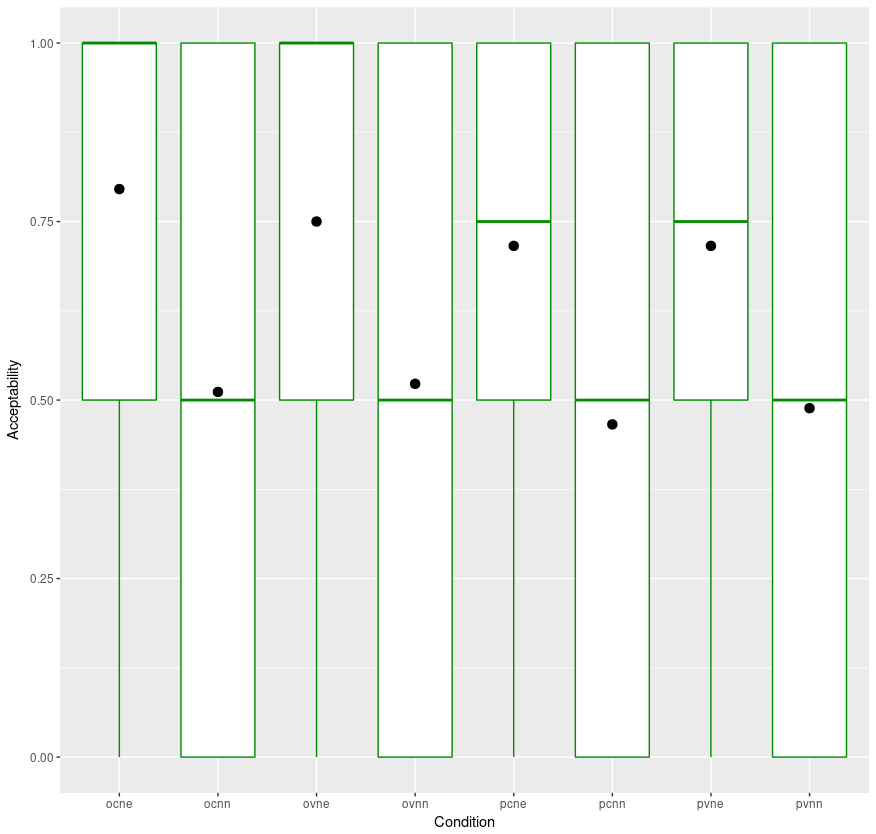
\includegraphics[width=.9\linewidth]{figures/Rplot10.png}
\centering
\caption{Means of responses average per subject and conditions \REF{ex:pcn}--\REF{ex:pvn}, \REF{ex:ocn}--\REF{ex:ovn} depending on their sub-conditions \REF{ex:wine_e}--\REF{ex:wine_n}, \REF{ex:rose_e}--\REF{ex:rose_n} (on the scale 0: inappropriate, 1: appropriate)}
\label{fig:graf}
\end{figure}

\figref{fig:graf} shows that I did not find the expected interaction between \textsc{vn} and \textsc{cn}. The reference level for the \textsc{e} sub-condition is \textsc{pcne} condition and the following statistical output shows that all conditions \textsc{pcne, pvne, ocne, ovne} are statistically not distinguishable from each other: \textsc{pvne:} $t= 0, p = 1$; \textsc{ocne:} $t=-1.226,p = 0.222$; \textsc{ovne:} $t = -0.509, p = 0.612$. The reference level for the \textsc{n} sub-condition is \textsc{pcnn} condition and all conditions \textsc{pcnn, pvnn, ocnn, ovnn} are statistically not distinguishable from each other again. The statistical output is the following: \textsc{pvnn:} $t = 0.300, p = 0.764$; \textsc{ocnn:} $t = -0.600, p = 0.549$; \textsc{ovnn:} $t = -0.751, p = 0.454$. The formal statistical results report no expected interaction between \textsc{cn} and \textsc{vn} conditions.

The experiment provides the following evidence on the discussed interaction in \ili{Czech}:

\begin{itemize}
\item[(\textsc{a})] \figref{fig:graf} shows that the acceptability rates of sentences with a \isi{comparative} in a \isi{predicate position} and the acceptability rates of sentences with a \isi{comparative} in an \isi{object position} are comparable. It does not support the assumption that the \isi{syntactic position} of a \isi{comparative} affects the acceptability of negated comparatives under a particular reading
(but see \citealt{kadmon2001formal}).

\item[(\textsc{b})] \textsc{cn-}comparatives and \textsc{vn-}comparatives are comparable.

\item[(\textsc{c})] The acceptability of all four conditions was higher in the equality sub-condition (\textsc{e}) than in the interval sub-condition (\textsc{n}).
\end{itemize}

\noindent The experimental results show that both \ili{Czech} \textsc{cn-} and \textsc{vn-}comparatives prefer the \isi{equality reading}; therefore they do not confirm the initial hypothesis that \ili{Czech} \textsc{cn-}comparati\-ves lead to the preferential \isi{interval reading}. Now I turn to the questions: (i) the correlation between \isi{focus} and two interpretations in \ili{Czech}, and (ii) reasons leading to two readings of \ili{Czech} \textsc{vn-}comparatives.


\section{Analysis and discussion}

\subsection{Czech \textsc{cn-}comparatives}\label{sect:ccn}

The statistical outputs show that sentences with \textsc{cn-}comparatives and \textsc{vn-}com\-pa\-ra\-tives are ambiguous between the \isi{equality reading} and the \isi{interval reading}, but both \isi{comparative} constructions prefer the \isi{equality reading}. The crucial point is that the results from the experiment go against Dočekal's claim that \textsc{cn-}comparatives show a preference for the \isi{interval reading}, but I agree with him that \ili{Czech} \textsc{cn} is a \isi{focus} operator that has to c-command its \isi{focus} marked constituent and has to be adjacent to the \isi{focus} marked constituent.

Previously, \citet{cohen2014superlative} and \citet{geurts2007least} observed that comparatives associate with \isi{focus}, which can lead to different truth-conditions depending on the focused element. Comparative modifiers like \textit{more than} may \isi{focus} varying portions of a sentence, as in \REF{ex:apples}.

\ea \label{ex:apples}
\ea Ann ate more than [two]$_{\textsc{foc}}$ apples. \label{ex:apples_int}
\ex Ann ate more than [two apples]$_{\textsc{foc}}$. \label{ex:apples_exh}
\z
\z

\noindent The sentence with \isi{comparative} modifiers may have two readings depending on the part of the sentence which is focused. \citet{geurts2007least} observed that \REF{ex:apples_int} implies that the number of apples that Ann ate exceeds two:  `Ann ate more than two apples, actually she ate four.' \REF{ex:apples_exh} implies that the number of apples that Ann ate was exactly two: `Ann ate more than two apples, she ate two apples, one pear, and two strawberries.' In the first case, we count how many apples Ann ate, but in the second case, we count how much of everything she ate.

I contend that what we observe in \ili{Czech} is the same phenomenon as already observed by \cite{dovcekal2017upper}, namely that the \isi{comparative} marker \textit{než} ‘than’ can have the equality or \isi{interval reading}. I add to this an observation that focusing of the \isi{numeral} would lead to the \isi{interval reading} only (the presupposed alternatives then are a set of integers $\{0,1\})$. However, because in \ili{Slavic} languages the \isi{focus} operator mainly appears adjacent to the focused element, the \isi{focus} on the \isi{comparative} marker \textit{než} signaling the \isi{equality reading} (and marginally \isi{interval reading}) is more salient, which can explain the preference observed in the experiment. Unfortunately, the experiment was a reading task; it did not control for the use of intonation.


\subsection{Czech \textsc{vn-}comparatives}

The experimental results support Dočekal's assertion that sentences with \textsc{vn-}comparati\-ves indeed lead primarily to the \isi{equality reading}, but the \isi{interval reading} is also possible.

At this point, I agree with Nouwen's line of argumentation that a narrow scope of \textsc{vn} \REF{ex:e_exh} denies a constituent, and a sentence can have the \isi{equality reading} because: (i) the number is bounded, and (ii) scalar implicatures are present; therefore they can be negated, and the truth condition is strengthened.

\ea  John did not find more than 20 mushrooms.
	\ea $\cnst{max}_{\cnst{d}}\big(\lambda y\exists x[\#x=y \wedge \textsc{mushroom}(x) \wedge \textsc{find}(\textsc{John},x)]\big) \leq 20$ \label{ex:e_exh}
 \ex truth conditions: $\cnst{max}_{\cnst{d}}(\lambda d\,.\,$the number of mushrooms was $d)\leq 20$ \label{ex:tc}
	\ex \isi{SI}: $\neg\cnst{max}_{\cnst{d}}(\lambda d\,.\,$the number of mushrooms was $d)\leq 19$ \label{ex:si}
	\ex $\cnst{max}_{\cnst{d}}(\lambda d\,.\,$the number of mushrooms was $d) = 20$ \label{ex:max}
\z
\z

\noindent The wide scope of \textsc{vn} \REF{ex:e_int} denies the whole proposition and the equality interpretation cannot occur because (i) the number is unbounded, and (ii) truth conditions cannot be strengthened because no scalar implicatures arise. The wide scope of \textsc{vn} leads to the interval interpretation (20,$\infty$).

\ea  John did not find more than 20 mushrooms.
\ea $\neg \cnst{max}_{\cnst{d}}\big(\lambda y\exists x[\#x=y \wedge \textsc{mushroom}(x) \wedge \textsc{find}(\textsc{John},x)]\big) > 20$ \label{ex:e_int}
\z
\z

\subsection{Discussion}

The most salient reading, which \ili{Czech} speakers associate with both \textsc{cn-} and \textsc{vn-}compa\-ratives, is equality. I analyze it in \sectref{sect:ccn} as a result of a particular \isi{focus} strategy. But I did not control for the \isi{focus} strategies in the experimental design. This is naturally what I will try to address in the next experiment.

The experiment design would be similar to the experiment presented in this article. Participants would judge whether sentences fit a context. The experiment would test only \ili{Czech} \textsc{cn-}comparatives because \textsc{vn-}comparatives did not involve \isi{focus} alternatives. In order to investigate whether focused comparatives indeed influence the preferred reading, participants would read aloud the tested sentences. The utterances would be recorded and digitized. The appropriate comparison of focused \textsc{cn-}comparatives and unfocused \textsc{cn-}comparatives could clarify the issue of \isi{focus} and the two possible interpretations of \ili{Czech} \textsc{cn-}comparatives.\footnote{Thanks to an anonymous reviewer for raising this point.}


\section{Conclusion}
I investigated \ili{Czech} negated comparatives compared with \ili{English} negated comparatives. I started with the observation that \ili{English} negated comparatives lead to two interpretations with respect to the type of \isi{negation}, i.e., the preferred \isi{interval reading} in the case of \textsc{vn} and the \isi{equality reading} in the case of \textsc{cn} \citep{nouwen2008upper}.

I experimentally tested \ili{Czech} negated comparatives. Although the experiment to some extent supports Dočekal's observation \citep{dovcekal2017upper}, it also adds some interesting twists. The experimental results show that both \ili{Czech} \textsc{cn-/vn-}compa\-ratives are ambiguous between an \isi{equality reading} and an \isi{interval reading}, although they strongly prefer the equality interpretation.

Following an approach that unifies scalar alternatives and \isi{focus} alternatives into one group and claims that both types of alternatives are the same (\citealt{katzir2007structurally,fox2011characterization,fox2018economy}), I argue that both \ili{Czech} \textsc{cn-}com\-par\-a\-tives and \ili{English} \textsc{cn-}comparatives result in the preference for \isi{equality reading} because they activate alternatives.

\ili{Czech} \textsc{vn-}comparatives behave in the same way as \ili{English} \textsc{vn-}comparatives: a particular reading depends on whether \isi{negation} takes wide scope or a narrow scope with respect to a proposition. The narrow scope of \textsc{vn} results in a preference for the \isi{equality reading} in \ili{Czech}, whereas the wide scope of \textsc{vn} leads to the \isi{interval reading}.

\section*{Abbreviations}

\begin{tabularx}{.48\textwidth}{lX}
\textsc{1}&first person\\
\textsc{acc}&{accusative}\\
\textsc{cn}&constituent {negation}\\
\textsc{dat}&{dative}\\
\textsc{e}&{equality reading}\\
\textsc{foc}&{focus}\\
\textsc{gen}&genitive\\
\textsc{inf}&{infinitive}\\
\textsc{ins}&instrumental\\
\textsc{loc}&locative\\
\end{tabularx}
\begin{tabularx}{.48\textwidth}{lX}
\textsc{n}&{interval reading}\\
\textsc{neg}&{negation}, negative\\
\textsc{nom}&nominative\\
\textsc{pl}&plural\\
\textsc{prs}&present\\
\textsc{pst}&past\\
\textsc{sg}&singular\\
\textsc{si}&{scalar implicature}\\
\textsc{vn}&{verbal negation}\\
&\\
\end{tabularx}

\section*{Acknowledgements}
The article improved in reaction to many questions and comments raised by two anonymous reviewers whom I want to thank very much. I would like to thank the audience at the very nice FDSL 12.5 conference that was held at University of Nova Gorica. Many thanks go to Marcin Wągiel for helping me with the second version of the article. I wish also to thank Mojmír Dočekal. I am happy to acknowledge that the research was supported by the Department of Linguistics and Baltic Languages at the Masaryk University in Brno (MUNI/A/0831/2016).



\sloppy
\printbibliography[heading=subbibliography,notkeyword=this]

\il{Czech|)}
\end{document}
